\section{Krzysztof Czerenko}
\label{sec:krzyczer}

overleaf-github integration

\begin {flushleft}
\textbf{Lorem ipsum} dolor sit amet, consectetur adipiscing elit. Maecenas tempus faucibus augue, dignissim placerat justo tempus id. Sed quis pharetra diam, id luctus metus. Vivamus dapibus arcu et nibh faucibus, id pharetra leo facilisis. Praesent non purus mauris. Quisque a nunc dignissim, imperdiet nulla at, auctor tellus. Aenean finibus magna erat, vel rhoncus lacus sodales non. Nullam eget velit quis mi egestas tincidunt a euismod nisl. Praesent non porta arcu. Vivamus dictum pretium leo. \underline{Aenean feugiat dolor diam, et scelerisque velit euismod sit amet.}\par
\end {flushleft}

\begin {center}
\textit{Cras placerat nulla at est sagittis cursus. Aenean maximus iaculis purus vitae pretium. Vivamus quis pretium justo. Quisque at sapien volutpat, pellentesque diam id, lacinia leo. Nulla laoreet lorem eget turpis faucibus interdum. Nullam sed sem placerat, pretium velit id, rutrum eros. Fusce vulputate mi at orci interdum auctor.Morbi lobortis varius leo. Maecenas pulvinar sodales massa eu fringilla.}\par
\end{center}

\vspace{2em}

To jest zdjęcie pandy. (zobacz zdjęcie~\ref{fig:panda}).

\vspace{2em}

\begin{figure}[htbp] 
    \centering
    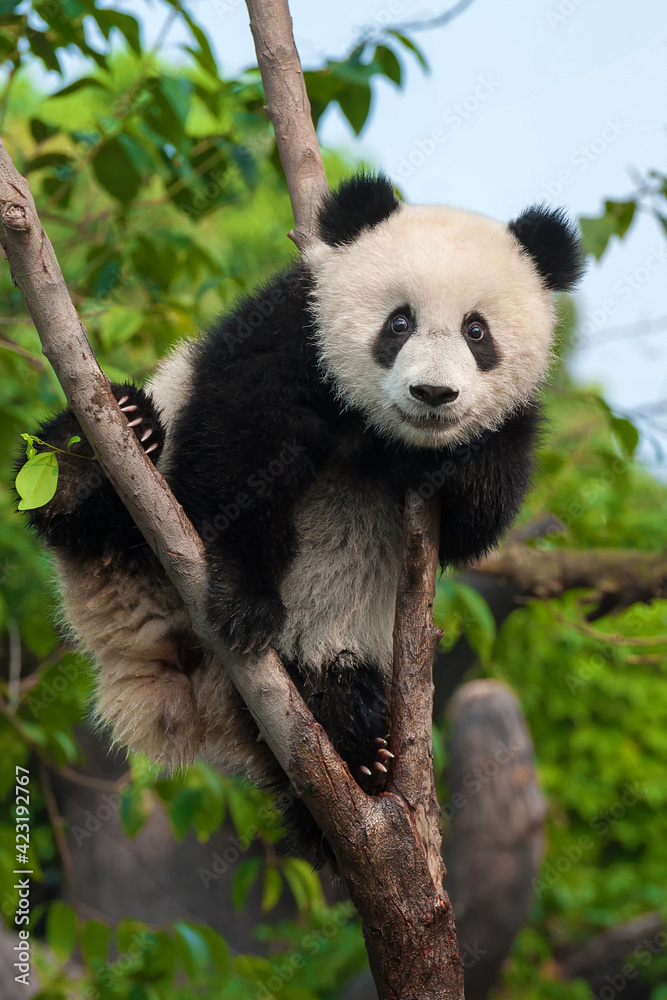
\includegraphics[width=0.2\textwidth]{pictures/baby_panda.jpg} 
    \caption{Ta panda jest słodka.}
    \label{fig:panda}
\end{figure}

\vspace{2em}

Tabela~\ref{tab1} to przykładowa tabela. 

\begin{table}[h]
\begin{tabular}{|
>{\columncolor[HTML]{FFC702}}c |cccclll|}
\hline
{\color[HTML]{3531FF} Lp.} & \multicolumn{7}{c|}{\cellcolor[HTML]{FFFFC7}\textbf{Example Table}}                                                                                                                         \\ \hline
1                          & \multicolumn{1}{c|}{item1}         & \multicolumn{1}{c|}{item2} & \multicolumn{1}{c|}{item3} & \multicolumn{1}{c|}{item4} & \multicolumn{1}{l|}{item5} & \multicolumn{1}{l|}{item6} & item7 \\ \hline
2                          & \multicolumn{1}{c|}{\textit{1000}} & \multicolumn{1}{c|}{2000}  & \multicolumn{1}{c|}{3000}  & \multicolumn{1}{c|}{4000}  & \multicolumn{1}{l|}{5000}  & \multicolumn{1}{l|}{6000}  & 7000  \\ \hline
\end{tabular}
\centering
\label{tab1}
\caption{Ta tabela jest ładna.}
\end{table}

\vspace{2em}

To jest równanie na postać trygonometryczną liczby zespolonej:
$$z = a + bi = \sqrt{a^2 + b^2}(\frac{a}{\sqrt{a^2 + b^2}} + i \frac{b}{\sqrt{a^2 + b^2}})$$

\vspace{2em}


Top 2 pandy:
\begin{enumerate}
    \item Kung-Fu Panda
    \item Baby Panda
\end{enumerate}


\vspace{2em}


Gatunki pand:
\begin{itemize}
    \item[-] panda wielka
    \item[-] panda ruda
\end{itemize}



